\documentclass{standalone}
\usepackage{tikz}
\usetikzlibrary{positioning, arrows.meta, calc}
\begin{document}




\newcommand{\waterlevel}[2]{
    \begin{scope}[shift={(#1,#2)}]
        \draw[line width=1pt] (-0.3, 0) -- (0.3, 0);
        \draw[line width=1pt] (0, 0) -- (-0.15, 0.25) -- (0.15, 0.25) -- cycle;
        \draw[line width=1pt] (-0.2, 0.25) -- (0.2, 0.25);
        \draw[line width=1pt,rotate=90,xshift=-4pt,yshift=-10.2pt] (-0.15, 0.4) .. controls (-0.05, 0.4) and (0.05, 0.3) .. (0.15, 0.4);
    \end{scope}
}

% Macro for a vertical valve (Bow-tie with T-handle)
\newcommand{\valveV}[2]{
    \begin{scope}[shift={(#1,#2)}]
        \draw[line width=1pt, fill=white] (-0.2, -0.3) -- (0.2, 0.3) -- (-0.2, 0.3) -- (0.2, -0.3) -- cycle;
        \draw[line width=1pt] (0, 0) -- (0.4, 0);
        \draw[line width=1pt] (0.4, -0.15) -- (0.4, 0.15);
    \end{scope}
}


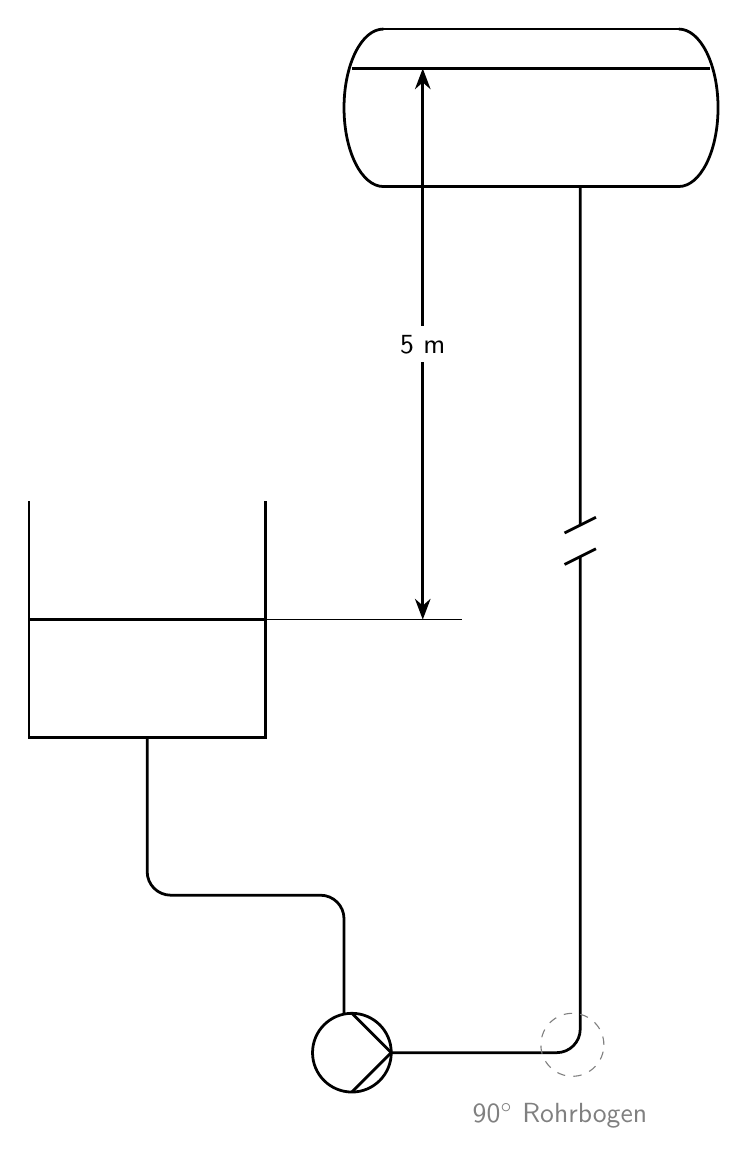
\begin{tikzpicture}[>=Stealth, font=\sffamily, line width=1pt]

% --- Colors for handwritten notes ---
\colorlet{pencolor}{black!50}

% --- Macros ---
% Macro for the water level symbol


% --- Tanks ---
% Tank 1 (Left, open)
\draw (0, 3) -- (0, 0) -- (3, 0) -- (3, 3);
\draw (0, 1.5) -- (3, 1.5); % Water surface
\waterlevel{1.5}{1.5}


% Tank 2 (Right Top, closed cylinder)
\begin{scope}[shift={(7, 8)}]
    \draw (-2.5, -1) -- (1.25, -1);
    \draw (-2.5, 1) -- (1.25, 1);
    \draw (-2.5, -1) arc (270:90:0.5 and 1);
    \draw (1.25, -1) arc (-90:90:0.5 and 1);
    
    \draw (-2.9, 0.5) -- (1.65, 0.5); % Water surface inside
    \waterlevel{1}{0.5}
%    \node[align=left] at (0, -0.2) {$p_B = 2 \text{bar}$\\ Überdruck};
\end{scope}

% --- Pipes ---
\draw (1.5, 0) -- (1.5, -1.7) -- (1.5, -1.7) to[bend right=45] (1.8, -2)--(3.7,-2) to[bend left=45] (4,-2.3) -- (4, -2.3)  -- (4, -3.7) to[bend right=45]  (4.3, -4);
% Path from Pump to Tank 2
\draw (4, -4) -- (6.7, -4) to[bend right=45] (7, -3.7)-- (7, 7);

% --- Pump ---
\draw[fill=white,xshift=-1.4cm] (5.5, -4) circle (0.5);
% Pump inner triangle symbol (flow direction)
%\draw (5.2, -4.2) -- (5.8, -4.2) -- (5.5, -3.6) -- cycle;
\draw[xshift=-1.4cm] (5.5,-3.5) -- (6,-4);
\draw[xshift=-1.4cm] (5.5,-4.5) -- (6,-4);

% --- Break in vertical pipe ---
\fill[white] (6.5, 2.3) rectangle (7.5, 2.7);
\draw (6.8, 2.2) -- (7.2, 2.4);
\draw (6.8, 2.6) -- (7.2, 2.8);

% --- Valves ---
\valveV{1.5}{-1}     % Under Tank 1
\valveV{4}{-3}       % Before Pump
\valveV{7}{-2.5}     % After Pump
\valveV{7}{6}        % Before Tank 2

% --- Dimensions and Labels ---
% 5m height dimension
\draw[thin] (3, 1.5) -- (5.5, 1.5);
\draw[<->] (5, 1.5) -- (5, 8.5) node[midway, fill=white] {5 m};


% "90° Krümmer" and circle
\node[pencolor, right] at (5.5, -4.8) {90$^\circ$ Rohrbogen};
\draw[pencolor, thin, dashed] (6.9, -3.9) circle (0.4); 



\end{tikzpicture}


\end{document}